%%%%%%%%%%%%%%%%%%%%%%%%
%
% $Autor: Malik Al Ashter Ghansletwala $
% $Datum: 2023-11-13  $
% $Directory: ML23-01-Keyword-Spotting-with-an-Arduino-Nano-33-BLE-Sense\report\Contents\en\HardwareDescription.tex $
% $Version: 4 $
% $Review by: Malik Al Ashter Ghansletwala$
% $Review date: 16.12.2023 $
%
%%%%%%%%%%%%%%%%%%%%%%%%

\chapter{Hardware Description}

Arduino stands as an open-source electronics platform, boasting adaptable and user-friendly hardware and software. Featuring on-board microcontroller and microprocessor kits, it facilitates the creation of both digital and analog devices. The microcontroller, often referred to as a miniature computer embedded on the Arduino board, typically requires additional electronic components such as diodes, resistors, capacitors, and transistors to manage voltage and current. However, the Arduino team has ingeniously designed a user-friendly environment to streamline hardware operation through software. Simply power the board to the required voltage, script the desired program, and upload it within seconds. This approach eliminates the need to grapple with intricate electronic configurations, granting independence from concerns about hardware intricacies.

As technological advancements in the semiconductor and electronics industry unfold, control problems are increasingly addressed using these compact microcontrollers instead of traditional mechanical and electrical switches. Across all Arduino boards, a common denominator is the microcontroller, essentially a diminutive computer pivotal in facilitating edge computing applications.\cite{Arduino:2023}

\section{Arduino Nano 33 BLE Sense}

The Arduino Nano Family encompasses a series of boards characterized by a compact footprint yet rich in features. This lineup spans from the economical entry-level Nano to the advanced Nano BLE Sense/Nano RP2040 Connect, incorporating Bluetooth/Wi-Fi radio modules. Additionally, these boards are equipped with an array of built-in sensors, including temperature, humidity, pressure, gesture, microphone, and more. Notably, they are programmable with MicroPython and are compatible with machine learning applications.\cite{Raj:2019}

The Arduino Nano 33 BLE Sense operates at a maximum of 3.3V, ensuring that its digital and analog pins are never subjected to higher voltages. Additionally, its Bluetooth Low Energy (BLE) module enhances its suitability for IoT applications. The board houses an nRF52840 processor with a clock speed of 64 megahertz, 256 kilobytes of Static RAM (SRAM), and 1 megabyte of flash memory. With 14 digital I/O pins, including eight analog input pins for external components and sensors, the board draws an impressively low 10 mA current per I/O pin.

\textbf{Dimensions:} \textit{The Arduino Nano 33 BLE Sense has precise dimensions of 45mm in lenght, 18mm in width, and its thickness is around 7mm.}

The nomenclature of the Arduino Nano 33 BLE Sense model itself conveys essential details. The designation "Nano" reflects its diminutive size, categorized as nano. Furthermore, the term "BLE" denotes support for Bluetooth Low Energy, while "Sense" indicates the incorporation of on-board sensors. These sensors encompass an accelerometer, gyroscope, magnetometer, temperature and humidity sensor, pressure sensor, proximity sensor, color sensor, gesture sensor, and even an integrated microphone.\cite{Raj:2019}

To enable RGB color analysis and person detection, it's essential to establish a connection between the BLE 33 Sense interface and the Arducam OV2640 camera shield. The Arducam OV2640 camera is employed for tasks such as RGB detection, object detection, and gesture recognition. The combination of the Arduino Nano 33 BLE Sense and the Arducam camera shield proves to be an ideal pairing for the development of machine learning (ML) and artificial intelligence (AI) applications. With a comprehensive set of on-board sensors, leveraging this setup involves the straightforward installation of relevant libraries on the Arduino board, seamlessly supporting the functionality of sensors and facilitating the implementation of machine learning applications.


The following figure shows top view and bottom view of Arduino Nano 33 BLE Sense, 

\begin{figure}[h!]
	\centering
	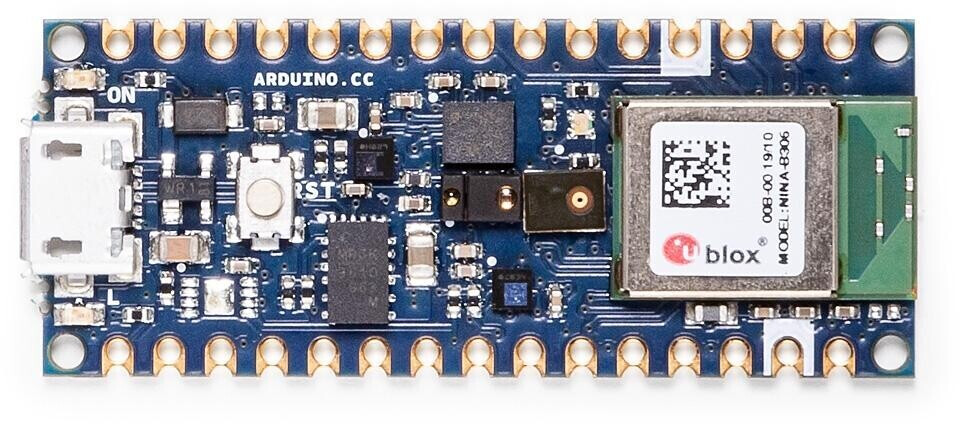
\includegraphics[width=0.6\textwidth]{Images/hardware/arduino-nano-33-ble-sense_1.jpg}
	\caption{Top view of Arduino Nano 33 BLE Sense} \label{fig:Arduino}
\end{figure}

\begin{figure}[h!]
	\centering
	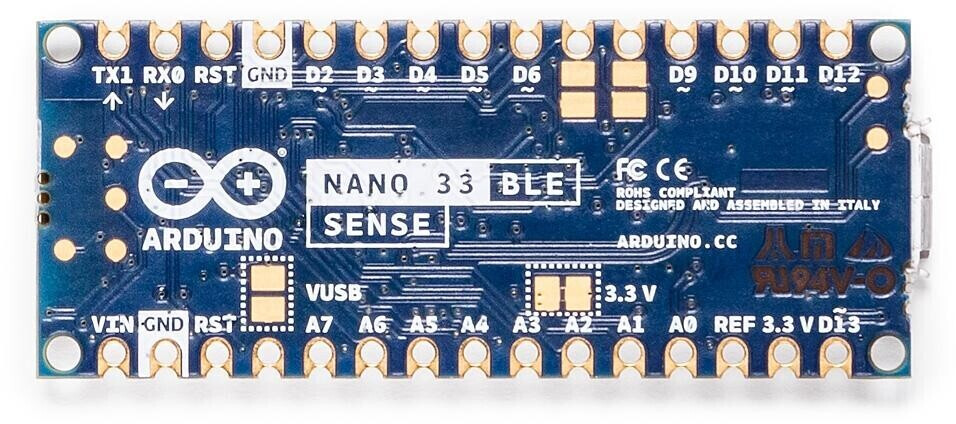
\includegraphics[width=0.6\textwidth]{Images/hardware/arduino-nano-33-ble-sense_2.jpg}
	\caption{Bottom view of Arduino Nano 33 BLE Sense} \label{fig:Arduino}
\end{figure}


The Nano board with Bluetooth Low Energy (BLE) capabilities is both compact and reliable, incorporating the NINA B306 module for BLE and Bluetooth 5 communication. This module is built on the Nordic nRF52480 processor, housing a robust Cortex M4F \ac{cpu}. The architecture seamlessly aligns with both Arduino IDE Online and Offline. The Arduino Nano BLE 33 Sense is equipped with a set of on-board sensors, namely ADPS-9960, LPS22HB, HTS221, LSM9DS1, and MP34DT05-A. Despite its small size, this board encompasses all the necessary sensors on board.
The Arduino Nano 33 BLE Sense have the following set of Sensors, BLE module and
its functionality below.\cite{Arduino:2023}

\begin{itemize}
	\item The Bluetooth is managed by a NINA B306 module.
	\item The ADPS-9960 is a digital proximity, ambient light, RGB and gesture sensor.
	\item The LSM9DS1 is a system-in-package featuring a 3D digital linear acceleration
	sensor, a 3D digital angular rate sensor, and a 3D digital magnetic sensor.
	\item The LPS22HB reads barometric pressure and environmental temperature.
	\item The MP34DT05 is support the sound detection.
	\item The HTS221 senses relative humidity.
\end{itemize}

\section{On-Board Sensor Description}

The Arduino Nano 33 BLE Sense is equipped with a range of embedded sensors on the board, commonly employed for measuring both analog and digital values in the surrounding environment. With compact dimensions of 45mm × 18mm, this board proves highly valuable for Internet of Things (IoT) and Artificial Intelligence (AI) applications, serving as an embedded device where space is a critical constraint. Operating at a low power consumption of 3.3V, this small-sized board can efficiently function on small batteries for extended periods, making it suitable for various applications.\cite{Arduino:2023}
Thanks to its onboard sensors, minimal power requirements, and compact architecture, the Nano board finds versatility in deployment. The Arduino Nano 33 BLE Sense introduces a new board on a familiar form factor. For in-depth information about each component and datasheets for individual sensors, detailed information can be accessed through the provided links. Brief descriptions of each sensor are outlined below.

\begin{itemize}
	\item The sensor MP34DT05 is the digital microphone. it is useful for capturing,
	analyzing and detecting the sound in real time. 
	\item The sensor HTS221 senses the relative humidity, and temperature, to get highly
	accurate measurements of the environmental conditions.
	\item The sensor LPS22HB is a barometric pressure sensor, it measures the environmental pressure which is usefull for simple weather station monitoring
	\item The sensor LSM9DS1 is a 9 axis Inertial Measurement Unit (IMU) use as
	a accelerometer, gyroscope, and magnatometer, this 9 axis sensor is ideal for
	wearable devices.
	\item The USB port allows you to connect Arduino Nano 33 BLE sense to your
	machine.
	\item The ADPS-9960 is a digital proximity, ambient light, RGB and gesture sensor.
	it can measure the proximity distance, light, color and gestures when moving
	close with the borad.
	\item There are 3 different LEDs that can be accessed on the Nano BLE Sense: RGB
	Programmable LED , the built-in orange Programmable LED and the Power
	LED.
\end{itemize}

Figure below illustrates the onboard embedded sensors, featuring a potent processor, the nRF52840 from Nordic Semiconductors. This processor stands out among other Arduino boards, boasting a 32-bit ARM® Cortex™-M4 \ac{cpu} running at 64 MHz. It's crucial to consider the accuracy of sensor readings, which heavily depends on the placement of the sensors within the environment. This aspect holds significant importance.

Furthermore, it's essential to note the operational conditions. The operating temperature should not surpass 85°C and should not fall below -40°C. Additionally, factors such as humidity levels and air pressure values should be carefully monitored.

\subsection{ Gesture, Proximity, and Color Detection Sensor ADPS-9960
}

The APDS-9960 device incorporates advanced features including Gesture detection, Proximity detection, Digital Ambient Light Sense (ALS), and Color Sense (RGB). Gesture detection employs four directional photodiodes to detect reflected infrared (IR) energy, emitted by the integrated LED. This process transforms physical motion information such as velocity, direction, and distance into digital data.\cite{Arduino:2023}

\begin{figure}[h!]
	\centering
	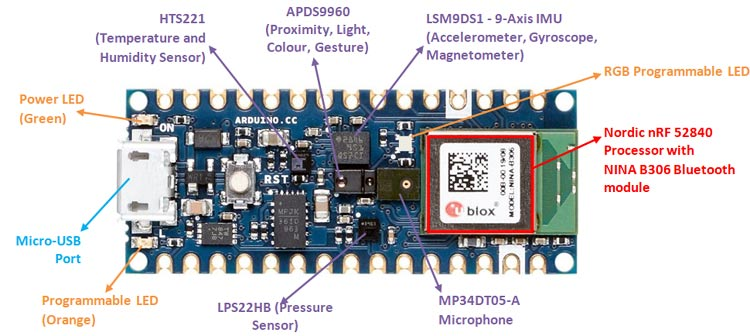
\includegraphics[width=0.6\textwidth]{Images/hardware/Arduino-Nano-33-BLE-Sense-Hardware-Overview}
	\caption{: Components in Arduino Nano 33 BLE Sense } \label{fig:Arduino}
\end{figure}

\begin{table}[ht]
	\centering
	\caption{Technical Specifications of Arduino Nano 33 BLE Sense}
	\begin{tabular}{|l|l|}
		\hline
		\textbf{Feature} & \textbf{Specification} \\
		\hline
		Microcontroller & nRF52840 \\
		Operating Voltage & 3.3V \\
		Input Voltage (Limit) & 21V \\
		DC Current per I/O Pin & 15 mA \\
		Clock Speed & 64MHz \\
		\ac{cpu} Flash Memory & 1MB \\
		SRAM & 256KB \\
		LED\_BUILTIN & 13 \\
		IMU (Accelerometer, Gyroscope, Magnetometer) & LSM9DS1 \\
		Microphone & MP34DT05 \\
		Gesture, Light, Proximity, Color Sensor & APDS9960 \\
		Barometric Pressure Sensor & LPS22HB \\
		Temperature, Humidity Sensor & HTS221 \\
		\hline
	\end{tabular}
	\label{tab:tech_specs}
\end{table}

For the following Applications the sensor is in use:

\begin{itemize}
	\item Gesture Detection
	\item Color Sense
	\item Ambient Light Sensing
	\item Proximity Sensing
\end{itemize}

\subsection{Accelerometer, Gyroscope, and Magnetometre Sensor
	LSM9DS1}

The LSM9DS1 is a system-in-package that integrates a 3D digital linear acceleration sensor, a 3D digital angular rate sensor, and a 3D digital magnetic sensor. Inertial Measurement Units (IMUs) operate by detecting rotational movements along three axes that is Pitch, Roll, and Yaw. This process relies on the collaboration of an Accelerometer, Gyroscope, and Magnetometer. The Accelerometer provides information about the velocity of the \ac{imu} module's movement. The Gyroscope measures the rate of rotational movement on the IMU. Additionally, the Magnetometer gauges the force of gravity acting on the \ac{imu}.

For the following Applications the IMU is in use:

\begin{itemize}
	\item Sports Technology - helping athletes to know how they can improve their
	movements.
	\item Compact transportation solutions like Segway.
	\item Consumer electronics; Smartphones, tablets, fitness trackers for motion sensing
	and orientation.
	\item Display/map orientation and browsing.
	\item Gaming and virtual reality input devices.
	\item Advanced gesture recognition.
	\item Indoor navigation.
\end{itemize}

Utilizing an Inertial Measurement Unit (IMU) comes with certain drawbacks and considerations. The primary drawback is the presence of accumulated error, commonly referred to as 'Drift.' This occurs due to the constant measurement of changes and the rounding off of calculated values. Over an extended duration, this process can result in notable errors. To mitigate the impact of drift, it is advisable to employ a high-quality IMU sensor and ensure proper calibration of the sensor.\cite{LSM9DS1:2015}


\subsubsection{Calibration of an IMU}

During the research, it was discovered that several methods exist for calibrating the involved sensors. The specific time intervals between each calibration are not explicitly defined; nevertheless, it is recommended to perform regular calibration, particularly when unusual outputs are observed\cite{Mallon:2015}. Below, we provide a brief overview of some calibration methods:


\subsubsection{Low and High Limit Method}

In this approach, the sensor undergoes circular rotations along each axis multiple times. The midpoint is subsequently determined between the two extremes. If there is no offset, the midpoint aligns closely with zero. However, if there is a slight deviation from zero, this value represents the hard iron offset, stemming from the distortion induced by the Earth's magnetic field. Primarily, this method is employed for calibrating the Magnetometer.\cite{Mallon:2015}


\subsubsection{Magneto V1.2}

In this technique, the raw magnetometer data undergoes pre-processing with axis-specific gain correction, transforming the raw output into nanoTesla.

\begin{center}
	\begin{verbatim}
		Xm_nanoTesla = rawCompass.m.x*(100000.0/1100.0);
		% Gain X [LSB/Gauss] for selected input field range
		Ym_nanoTesla = rawCompass.m.y*(100000.0/1100.0);
		Zm_nanoTesla = rawCompass.m.z*(100000.0/980.0);
	\end{verbatim}
\end{center}

This converted data is saved into the file  \texttt{Mag\_raw.txt} that you open with the Magneto program. To start using this method, we first need to replace the (100000.0/1100.0)
scaling factors with values that convert your specific sensors output into nanoTesla.
Rather than simply finding an offset and scale factor for each axis, Magneto creates
twelve different calibration values that correct for a whole set of errors: bias, hard
iron, scale factor, soft iron and misalignment.

An additional advantage of this method is its applicability for accelerometer calibration. Once again, you may need to preprocess the specific raw accelerometer output, considering factors such as bit depth and G sensitivity, to transform the data into milliGalileo. Subsequently, inputting a value of 1000 milliGalileo serves as the "norm" for the gravitational field.\cite{Mallon:2015}

\subsection{Pressure Sensor LPS22HB}

The LPS22HB serves as an ultra-compact piezoresistive absolute pressure sensor, operating as a digital output barometer. It finds application in the following scenarios:

\begin{itemize}
	\item Sports watches
	\item Altimeters and barometers for portable devices
	\item Weather station equipment
\end{itemize}

An installed sensor element, along with an IC interface, communicates through an I2C or SPI bus. Its functionality is specified within a temperature range from -40°C to +85°C.

\begin{itemize}
	\item Absolutdruckbereich: 260 bis 1260 hPa
	\item 16-bit Temperaturdatenausgabe
	\item Versorgungsspannung: 1,7 bis 3,6 Volt
	\item 24-bit Druckdatenausgabe
\end{itemize}

\subsection{Relative Humidity and Temperature Sensor HTS221}

The HTS221 is a highly compact sensor designed for measuring relative humidity and temperature. It incorporates a sensing element and a mixed signal to deliver measurement information via digital serial interfaces. This sensor is employed in the following applications:

\begin{itemize}
	\item Air conditioning, heating and ventilation
	\item Smart home automation
	\item Industrial automation
	\item Air humidifiers
	\item Refrigerators
\end{itemize}

This sensor communicates via the I2C and SPI buses. It is operational within a temperature range from -40°C to +120°C. Power supply in the range of 1.7 to 3.3 volts is required. Temperature measurement is conducted with an accuracy of ±5°C.

\begin{itemize}
	\item SDA/SDI/SDO - I2C serial Data (SDA) and 3 wire-SPI serial data input/output
	(SDI/SDO)
	\item  SCL/SPC - I2C serial clock (SCL) and SPI serial port clock (SPC)
	\item DRDY - Data ready output signal
	\item SPI enable - I2C/SPI mode selection
	\item VDD - Stromversorgung
	\item GND - Ground
\end{itemize}

\subsection{Digital Microphone MP34DT05-A}

The MP34DT05-A is a highly compact and energy-efficient digital microphone featuring omnidirectional capabilities. It incorporates a capacitive sensing element and an IC interface. The sensing element, designed for detecting acoustic waves, undergoes manufacturing through a specialized silicon micromachining process dedicated to audio sensor production. The MP34DT05 is characterized as a low-distortion microphone with a signal-to-noise ratio of 64 dB, a sensitivity of -26 dBFS ± 3 dB, and an Acoustic Overload Point (AOP) at 122.5 dBSPL. The microphone produces a PDM signal as its output, which is a binary signal modulated by Pulse Density Modulation (PDM) from the analog signal\cite{MP34DT06J:2021}. The sensor is utilized in the following applications:

\begin{itemize}
	\item Portable media player
	\item Mobile Terminal
	\item Speech recognition
\end{itemize}

\begin{figure}[h!]
	\centering
	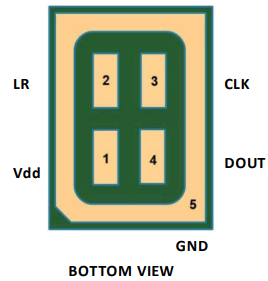
\includegraphics[width=0.6\textwidth]{Images/hardware/bottom-view}
	\caption{} \label{fig:Bottom view}
\end{figure}

\begin{figure}[h!]
	\centering
	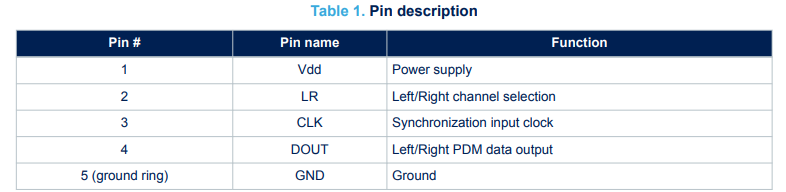
\includegraphics[width=1.3\textwidth]{Images/hardware/pin-description}
	\caption{Circuit diagram microphone} \label{fig:Pin description}
\end{figure}\cite{MP34DT06J:2021}

\subsection{Bluetooth Module nRF52840}

The nRF52840 stands as an advanced and exceptionally versatile single-chip solution tailored to meet the growing demands of Ultra Low Power (ULP) wireless applications. This includes devices in close proximity, connected living environments, and the broader realm of the \ac{iot} \cite{Arduino:2023}. Specifically designed to accommodate major feature advancements of Bluetooth 5, it leverages the enhanced performance capabilities introduced by Bluetooth 5.

\textbf{ Applications:}
 
 \begin{itemize}
 	\item Connected Health
 	\item Wearables with wireless payment
 	\item Advanced personal fitness devices
 	\item Connected watches
 	\item Smart city infrastructure
 	\item Industrial mesh networks
 	\item Smart Home products 	
 \end{itemize}
 
 \section{Arduino Nano 33 BLE Pin Configuration}
 
 The Arduino Nano 33 BLE represents an advanced iteration of the Arduino Nano board, employing the robust nRF52840 processor. As illustrated in Figure 2.4, the board exhibits the subsequent pin configuration:
 
 \textbf{Digital Pins:} There are 14 digital I/O pins that exclusively receive either HIGH or LOW values. These pins function as either input or output based on specific requirements. A HIGH state is achieved when the pins receive 5V, while a LOW state corresponds to a reception of 0V.
 
 \textbf{Analog Pins:} The board boasts a total of 8 analog pins labeled A0 to A7. In contrast to digital pins, these analog pins can receive a range of values. They are instrumental in measuring analog voltages spanning from 0 to 5V.
 
\textbf{ PWM Pins:} All digital pins on the board can be utilized as PWM pins, generating analog results through digital means.
 
 \textbf{SPI Pins:} The board supports the serial peripheral interface (SPI) communication protocol, facilitating communication between the controller and peripheral devices such as shift registers and sensors. Two pins, Master Input Slave Output (MISO) and Master Output Slave Input (MOSI), are dedicated to SPI communication, facilitating the exchange of data.
 
 \textbf{I2C Pins:} The board is equipped with the I2C communication protocol, a two-wire interface with SDL and SCL pins.
 
\textbf{ UART Pins:} Featuring the UART communication protocol for serial communication, the board includes Rx and Tx pins. Rx serves as the receiving pin for serial data, while Tx functions as the transmission pin.
 
\textbf{ External Interrupts Pins:} All digital pins can function as external interrupts, allowing the interruption of the main program with specific instructions in emergency scenarios.
 
\textbf{ LED at Pin 13 and AREF Pin:} Pin 13 hosts an LED on the board, and AREF functions as a reference voltage for input voltage.

\begin{figure}[h!]
	\centering
	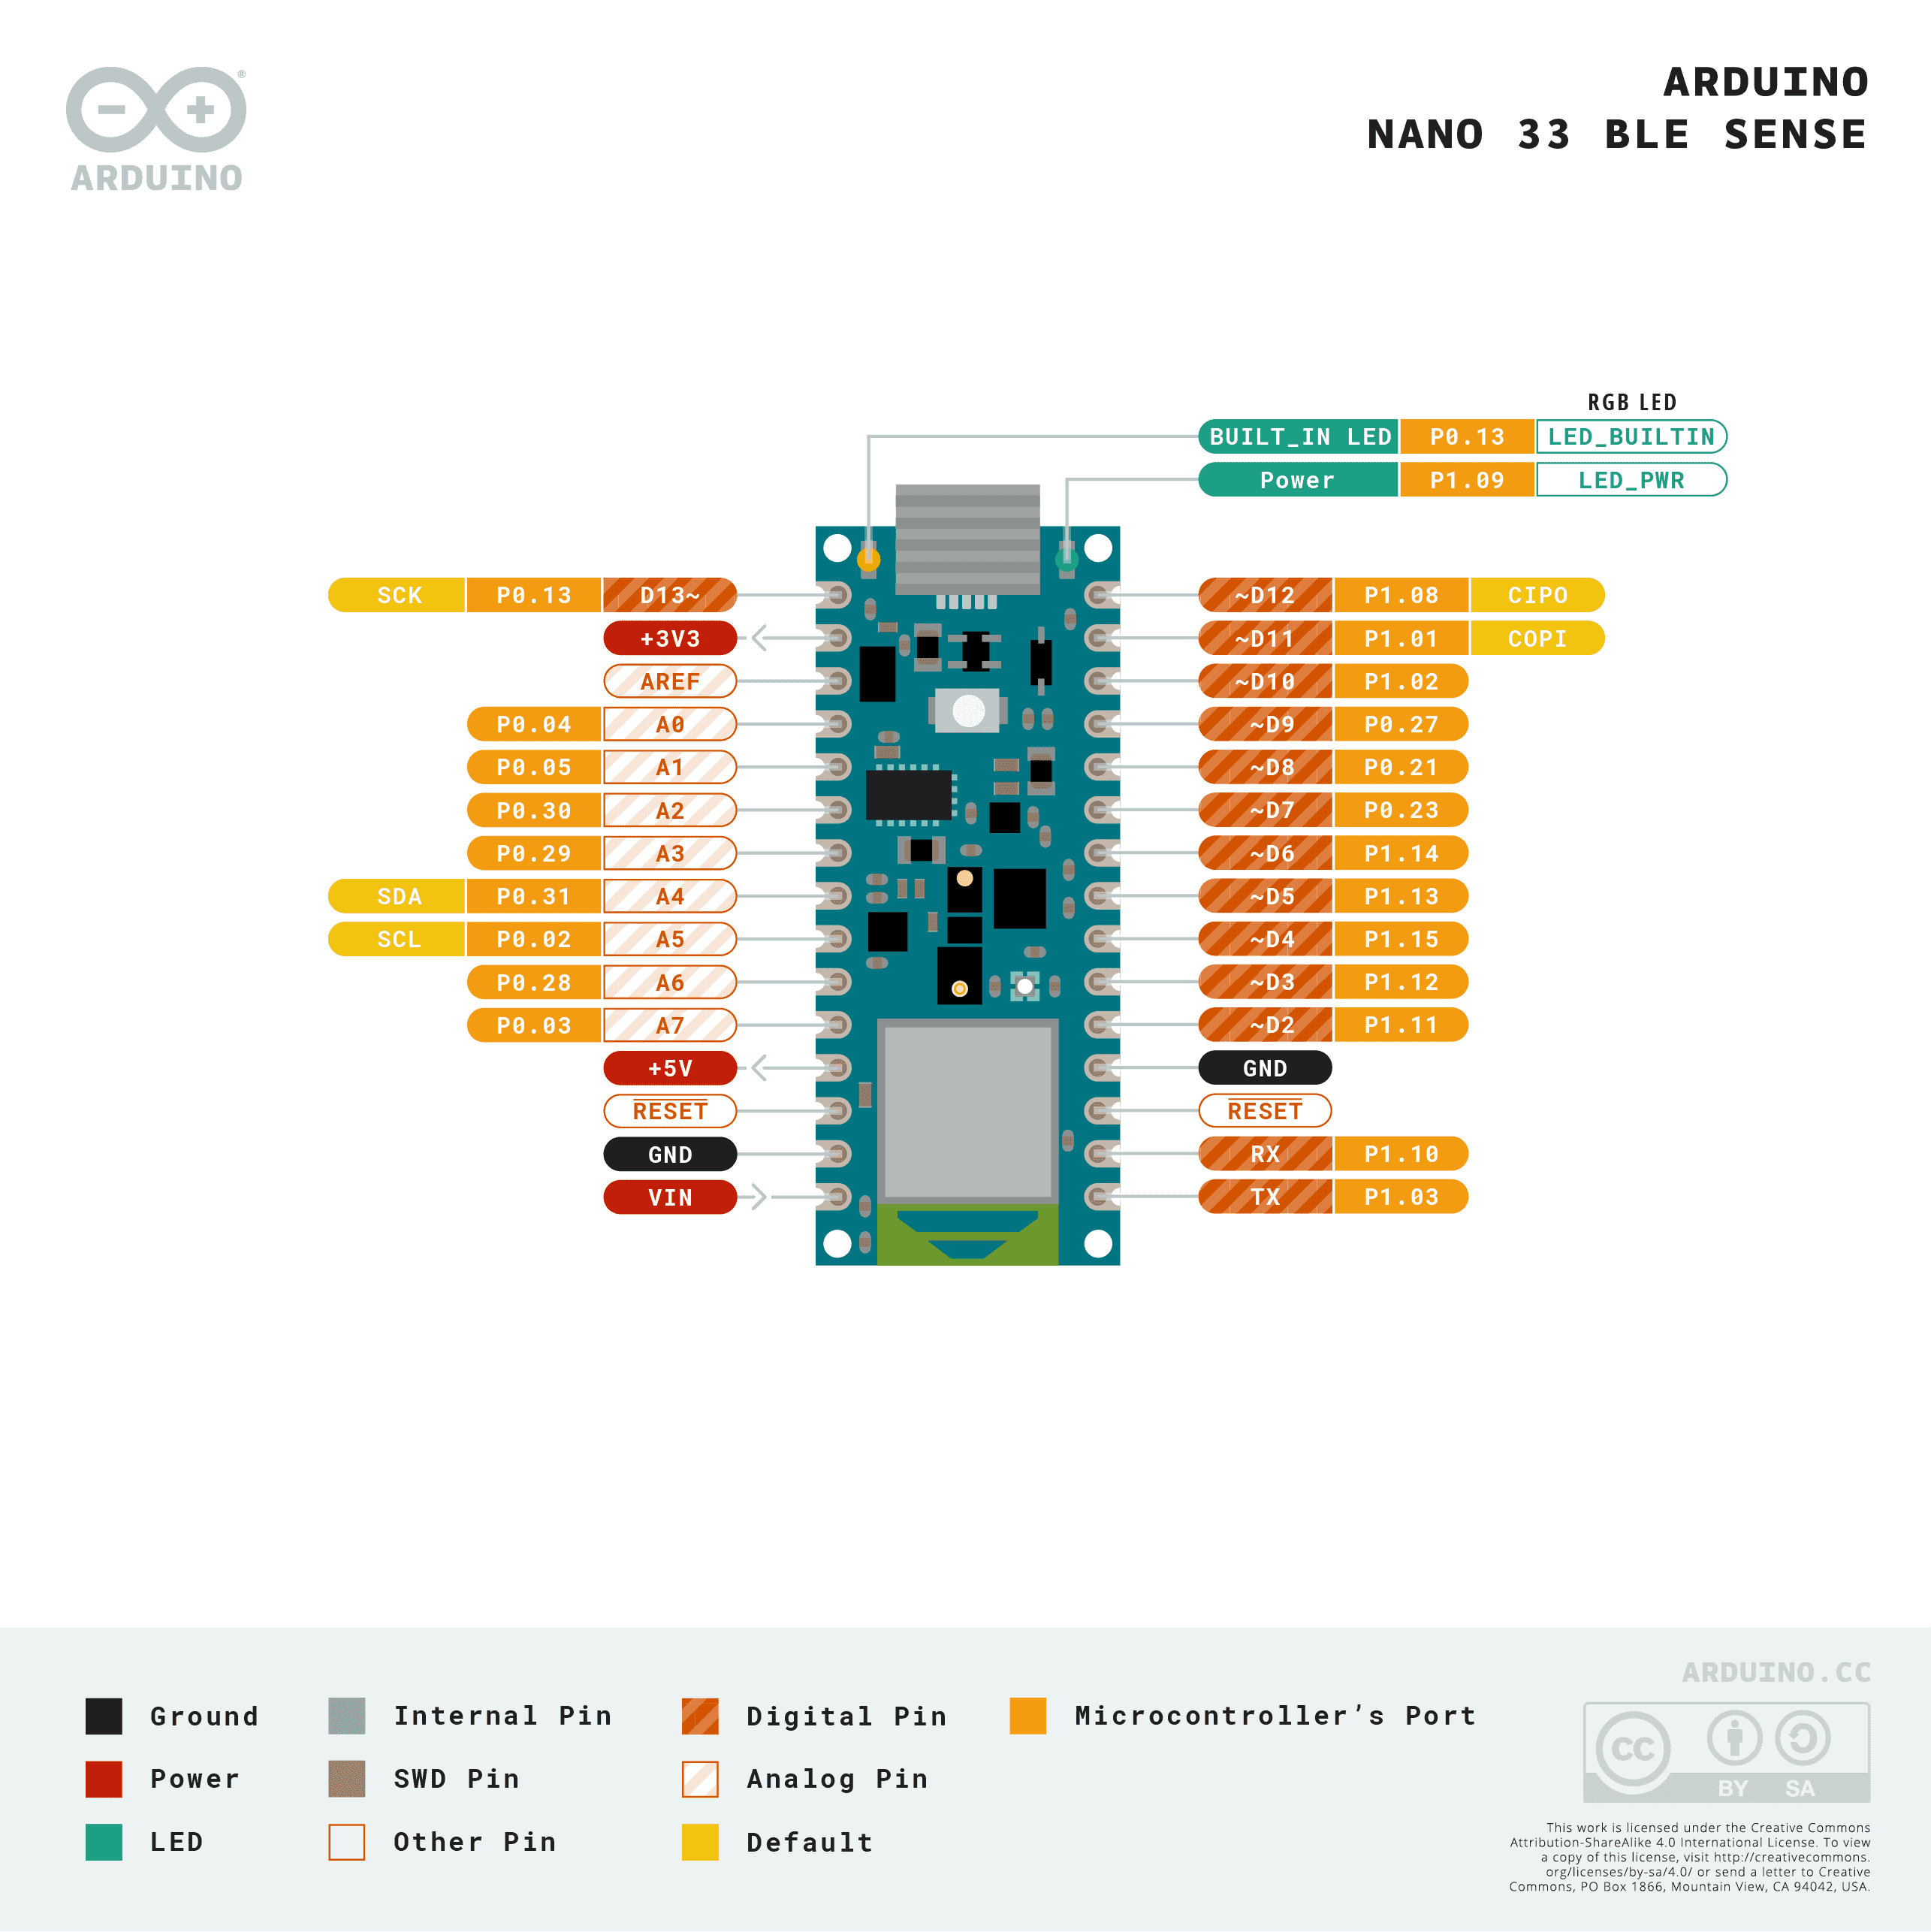
\includegraphics[width=1.1\textwidth]{Images/hardware/pinout}
	\caption{Arduino Nano 33 BLE Pin Configuration} \label{fig:pinout}
\end{figure}

\section{Hardware Tests}

All the Arduino boards need power to operate, either it comes from the USB connection
with Laptop, Ac power adapter, Battery or a regulated power supply. The most easiest
way to operate arduino board is USB connection with laptop, normally these boards
need 5V direct current (DC) to operate. Arduino Nano 33 BLE sense also need these
types of power sources for functionality, when applying one of the above mention power
source the green LED glows as shown in the figure 3.7, it shows the sign of Arduino
board working.

\begin{figure}[h!]
	\centering
	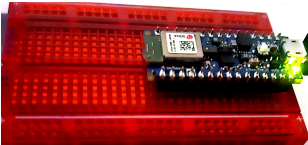
\includegraphics[width=0.6\textwidth]{Images/hardware/Power-On-Arduino-Nano-33-BLE-Sense}
	\caption{Power On Arduino Nano 33 BLE Sense} \label{fig:Power-On-Arduino-Nano-33-BLE-Sense}
\end{figure}

\subsection{Hardware parts}

The Arduino Nano 33 BLE Sense is equipped with a variety of hardware features that make it particularly suitable for projects involving keyword spotting. Here’s a breakdown of its relevant parts and it's functions and how they support the development and deployment of a keyword spotting application:

\begin{enumerate}
	\item \textbf{nRF52840 Microcontroller (MCU)}
	\begin{itemize}
		\item \textbf{Core Function:} This powerful ARM Cortex-M4 CPU runs at up to 64 MHz and is the brain of the Arduino Nano 33 BLE Sense. It's responsible for executing the code that processes input data, runs the machine learning (ML) model, and controls the output based on the model's inference.
		\item \textbf{Keyword Spotting Relevance:} The MCU performs the real-time signal processing and inference tasks required for keyword spotting. It has enough computational power to run lightweight TinyML models directly on the device.
	\end{itemize}	
	\item \textbf{Built-in LED:}
	\begin{itemize}
		\item\textbf{ Core Function:} The Arduino Nano 33 BLE Sense has a built-in RGB LED (Light Emitting Diode).
		\item \textbf{Keyword Spotting Relevance:} The LED can be used to provide visual feedback based on keyword detection. For our project, it can light up in different colors or patterns to indicate the recognition of specific keywords.
	\end{itemize}
	\item \textbf{ BLE (Bluetooth Low Energy) Capability:}
	\begin{itemize}
		\item \textbf{Core Function:} Allows wireless communication over Bluetooth.
		\item \textbf{Keyword Spotting Relevance:} This feature can be used to transmit the results of keyword spotting to other devices, such as smartphones, tablets, or computers. It enables the Arduino Nano 33 BLE Sense to function as part of a larger ecosystem, where it can send notifications or control other devices based on voice commands.
	\end{itemize}
	\item\textbf{ Digital Microphone (MP34DT05):}
	\begin{itemize}
		\item \textbf{Core Function:} This microphone captures audio signals, which are essential for any voice or sound-based application.
		\item\textbf{ Keyword Spotting Relevance:} It captures the user's keywords in the form voice commands. The audio data from the microphone is then processed and fed into the ML model for keyword detection.
	\end{itemize}
	
\end{enumerate}

\subsection{Hardware Functions}

\subsubsection{Test with MP34DT05 (Digital Microphone)}

Testing the MP34DT05 digital microphone on the Arduino Nano 33 BLE Sense for keyword spotting involves setting up the microphone, capturing audio data, and potentially sending the data to a keyword spotting model for analysis. The embed on-board MP34DT05 sensor in Arduino Nano 33 BLE Sense has the
funcnality to sense audio voice from the environment. There is build in Arduino
library for this particular sensor, which is PDM as shown in the figure.

\begin{figure}[h!]
	\centering
	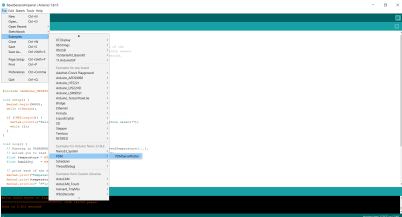
\includegraphics[width=0.6\textwidth]{Images/hardware/Digital-Microphone}
	\caption{MP34DT05, Digital Microphone} \label{fig:Digital-Microphone}
\end{figure}

\subsubsection{RGB LED pins on the Arduino Nano 33 BLE Sense}

\begin{code}[h!]
	\lstinputlisting[language=c, numbers=none, linerange={14-18}]{Code/testhardware/microphone.c}    
	\caption{RGB LED pins on the Arduino Nano 33 BLE Sense}
\end{code}

\subsubsection{Function to blink the LED with the specified color}

\begin{code}[h!]
	\lstinputlisting[language=c, numbers=none, linerange={19-30}]{Code/testhardware/microphone.c}    
	\caption{Function to blink the LED with the specified color}
\end{code}

\subsubsection{Initialization}

\begin{code}[h!]
	\lstinputlisting[language=c, numbers=none, linerange={31-53}]{Code/testhardware/microphone.c}    
	\caption{Initialization}
	\end{code}
	
\subsubsection{Classification Results}	

\begin{code}[h!]
	\lstinputlisting[language=c, numbers=none, linerange={55-64}]{Code/testhardware/microphone.c}    
	\caption{Classification Results}
\end{code}

\begin{itemize}
	\item \textbf{Setup Function:} 
	\begin{itemize}
		Initializes serial communication, configures the RGB LED pins as outputs, and initializes the Edge Impulse model with \texttt{Keywordspotting.begin()}. It checks for successful initialization of the model, halting the program if it fails.
	\end{itemize}
	\item \textbf{Loop Function}
	\begin{itemize}
		\item Runs the keyword spotting classifier with \texttt{Keywordspotting.run classifier(and result, false)} and checks the classifier's output.
		\item Depending on the classification result, it blinks the LED in green, red, or blue. The decision is made based on the confidence level of the classification for "yes" and "no". If neither confidence level is above 0.8, it defaults to blinking blue, indicating an unrecognized keyword.
	\end{itemize}
	\item \textbf{ Blink Function:}
	\begin{itemize}
		\item \texttt{blinkLED(int red, int green, int blue)} controls the RGB LED based on the specified color parameters. It turns on the LED with the color combination provided for half a second, then turns it off for half a second.
	\end{itemize}
	\item \textbf{ Considerations and Enhancements:}
	\begin{itemize}
		\item \textbf{ Model Indexing:} The code assumes that "yes" is at index 0 and "no" is at index 1 of the classification results. Ensure this aligns with how your model was trained and how the labels were indexed during the training process.
		\item \textbf{Model Initialization and Error Handling:} The \texttt{Keywordspotting.begin()} and classifier run check for initialization and execution errors, which is good practice for detecting and handling runtime issues.
	\end{itemize}
\end{itemize}

\subsection{Responses of the Device}

\begin{itemize}
	\item As mentioned in the code, the \texttt{Green LED} blinks whenever the keyword \texttt{YES} is produced in form of voice command.

\begin{figure}[h!]
	\centering
	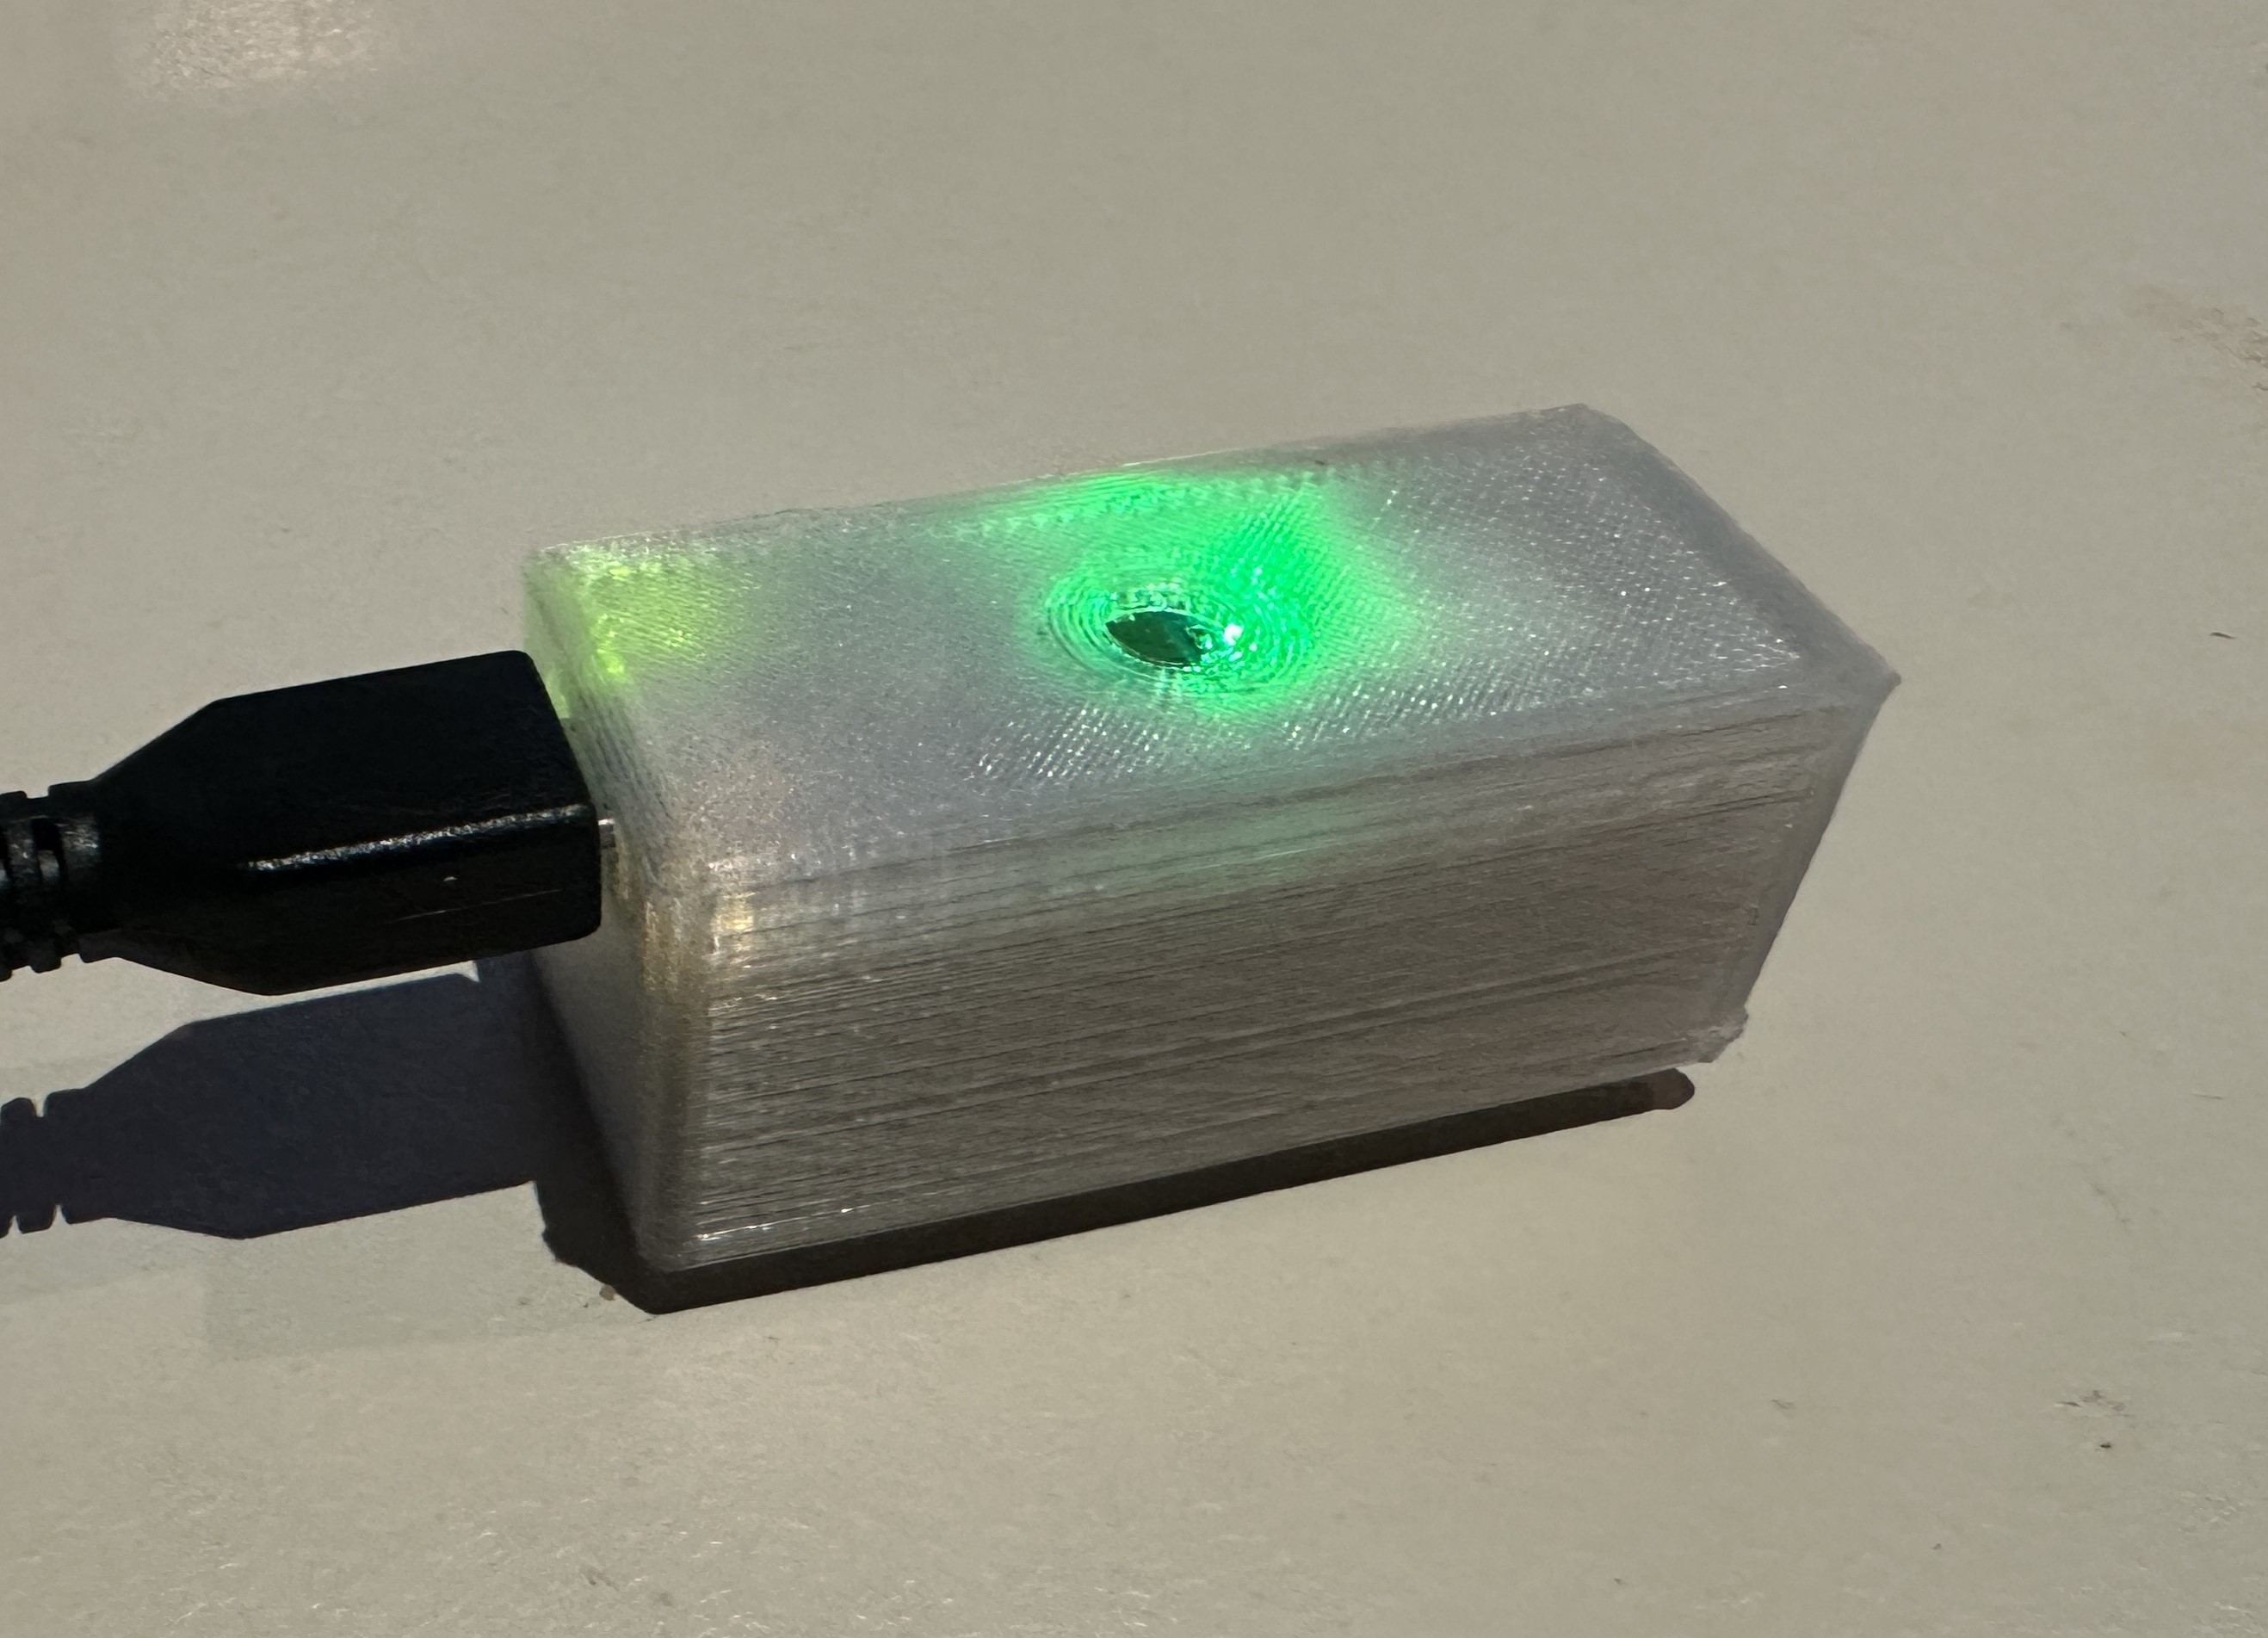
\includegraphics[width=0.6\textwidth]{Images/testhardware/ArduinoGreen}
	\caption{ Response to the
		keyword YES} \label{fig:ArduinoGreen}
\end{figure}

	\item  As mentioned in the code, the \texttt{RED LED} blinks whenever the keyword \texttt{NO} is produced in form of voice command.
	
	\begin{figure}[h!]
		\centering
		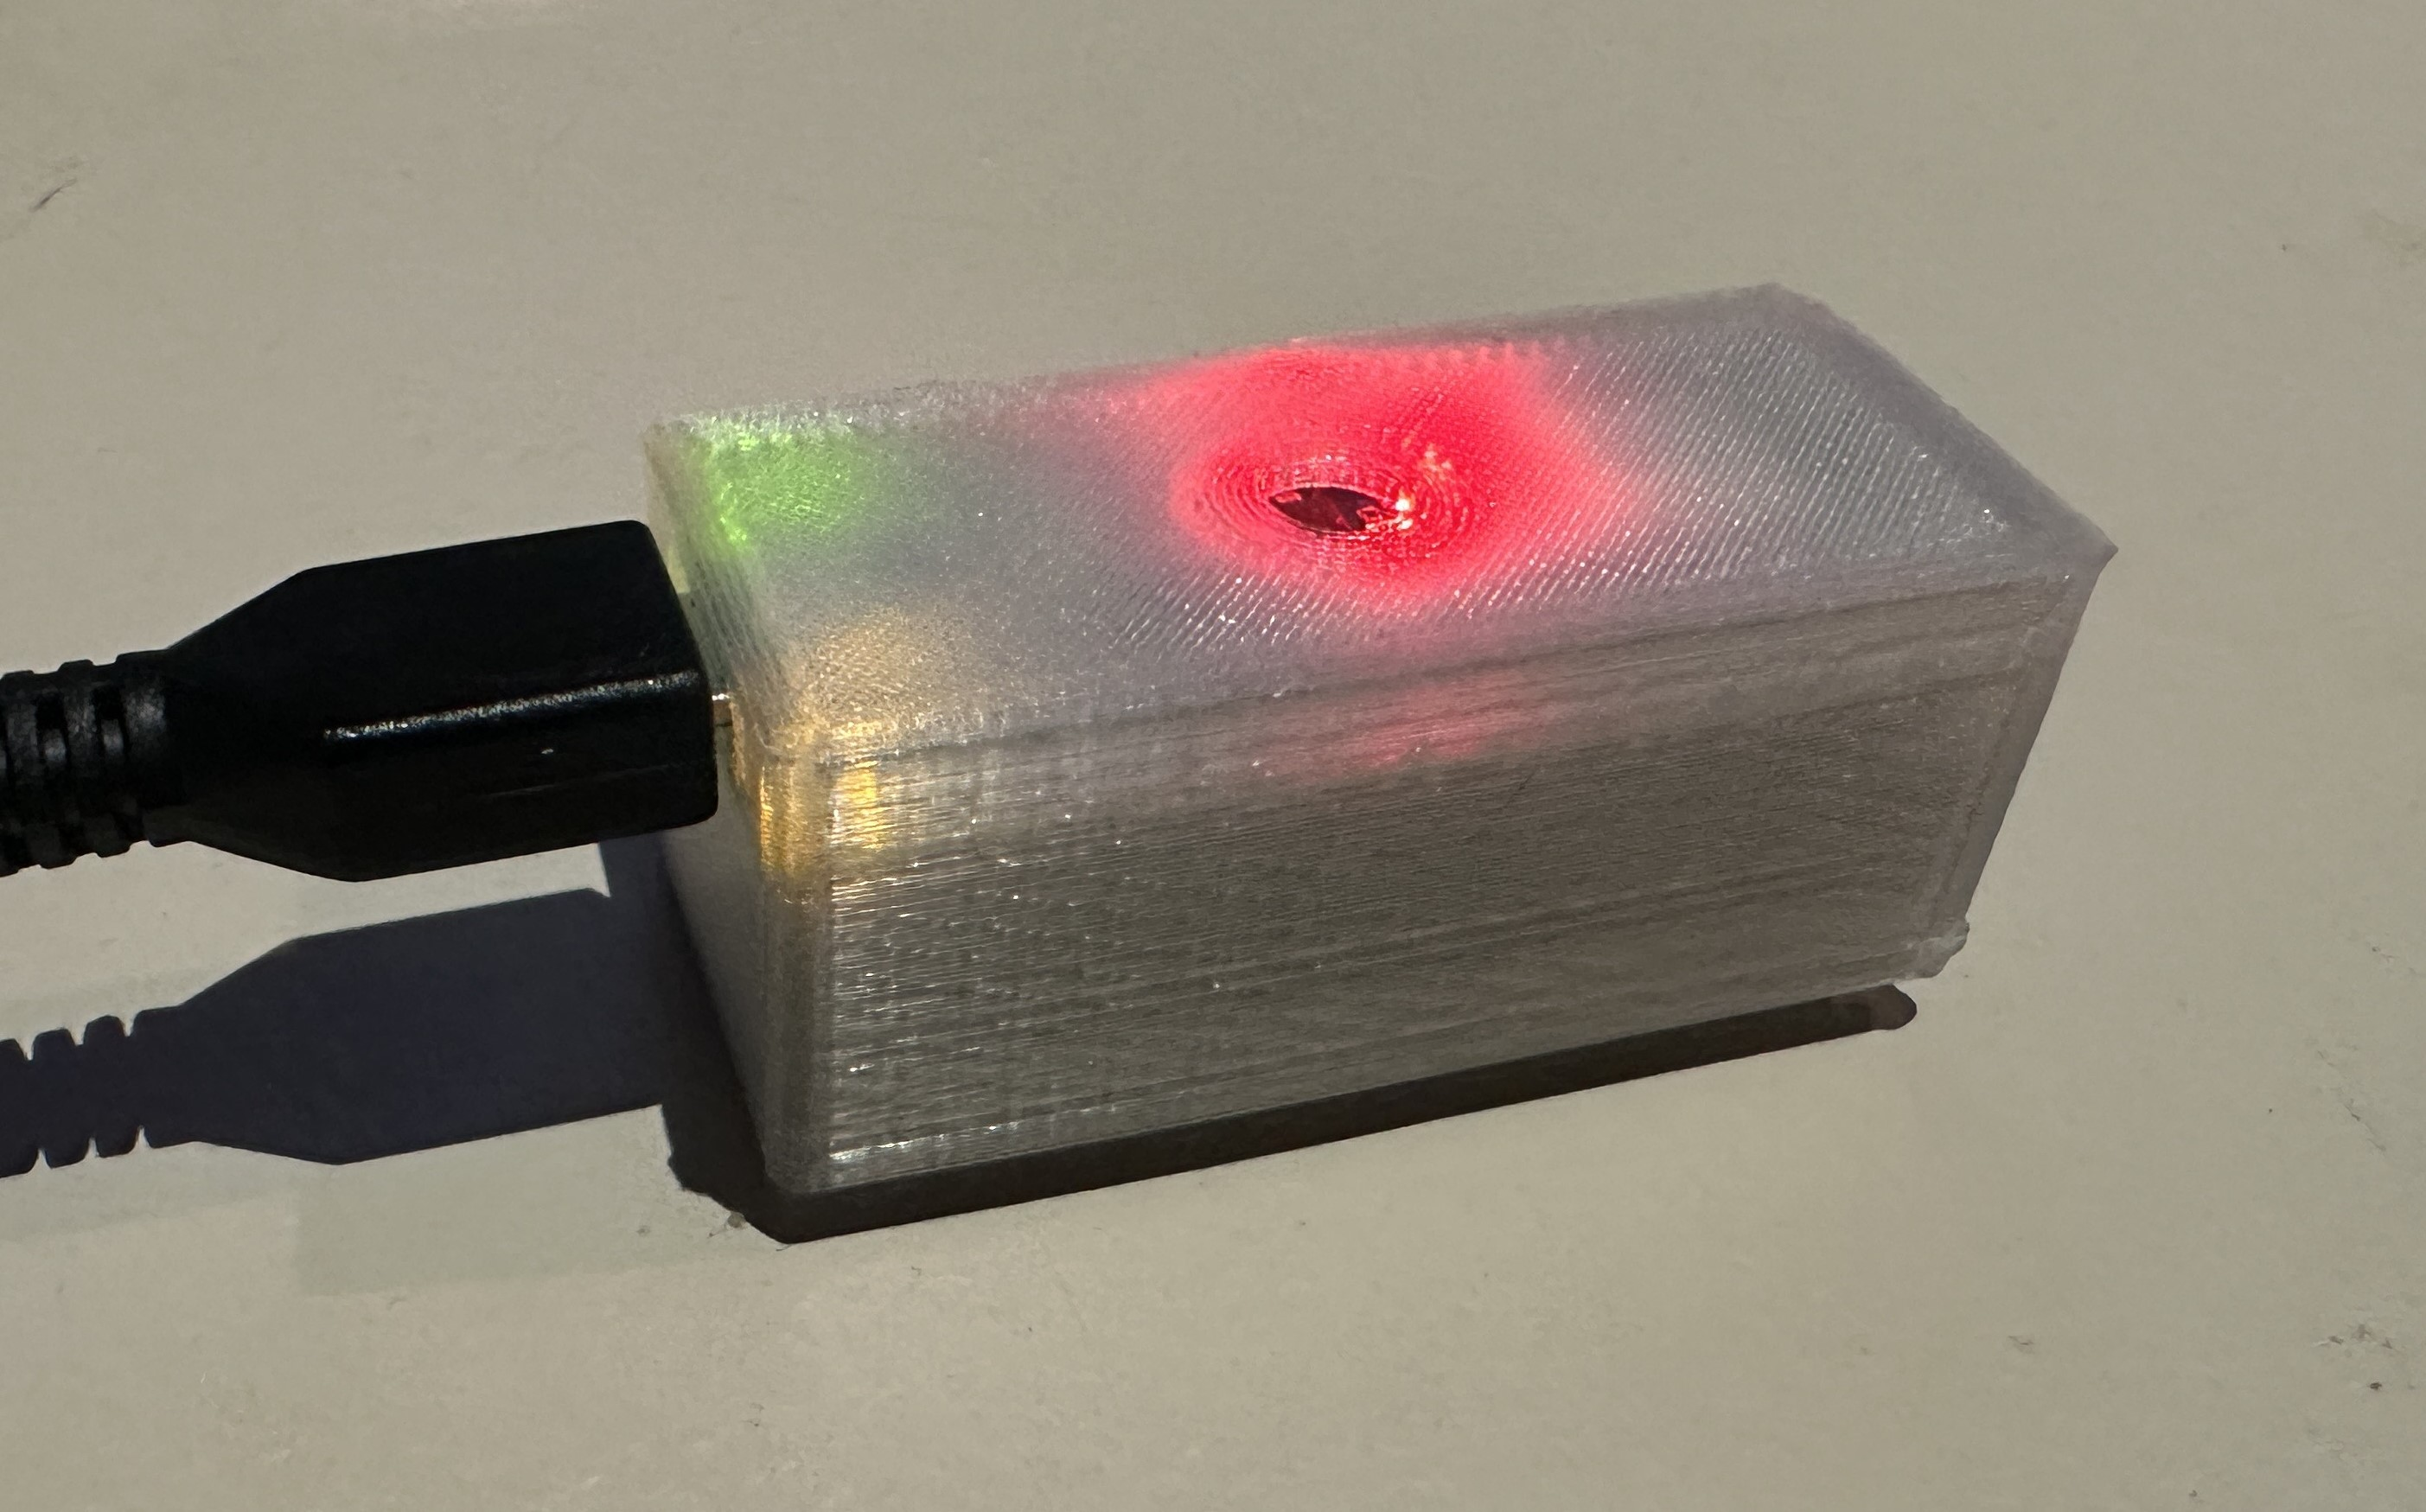
\includegraphics[width=0.6\textwidth]{Images/testhardware/ArduinoRed}
		\caption{ Response to the
			keyword NO} \label{fig:ArduinoRed}
	\end{figure}
	
		\item  As mentioned in the code, the \texttt{BLUE LED} blinks whenever \texttt{UNRECOGNIZED KEYWORD} is produced in form of voice command.
		
		\begin{figure}[h!]
			\centering
			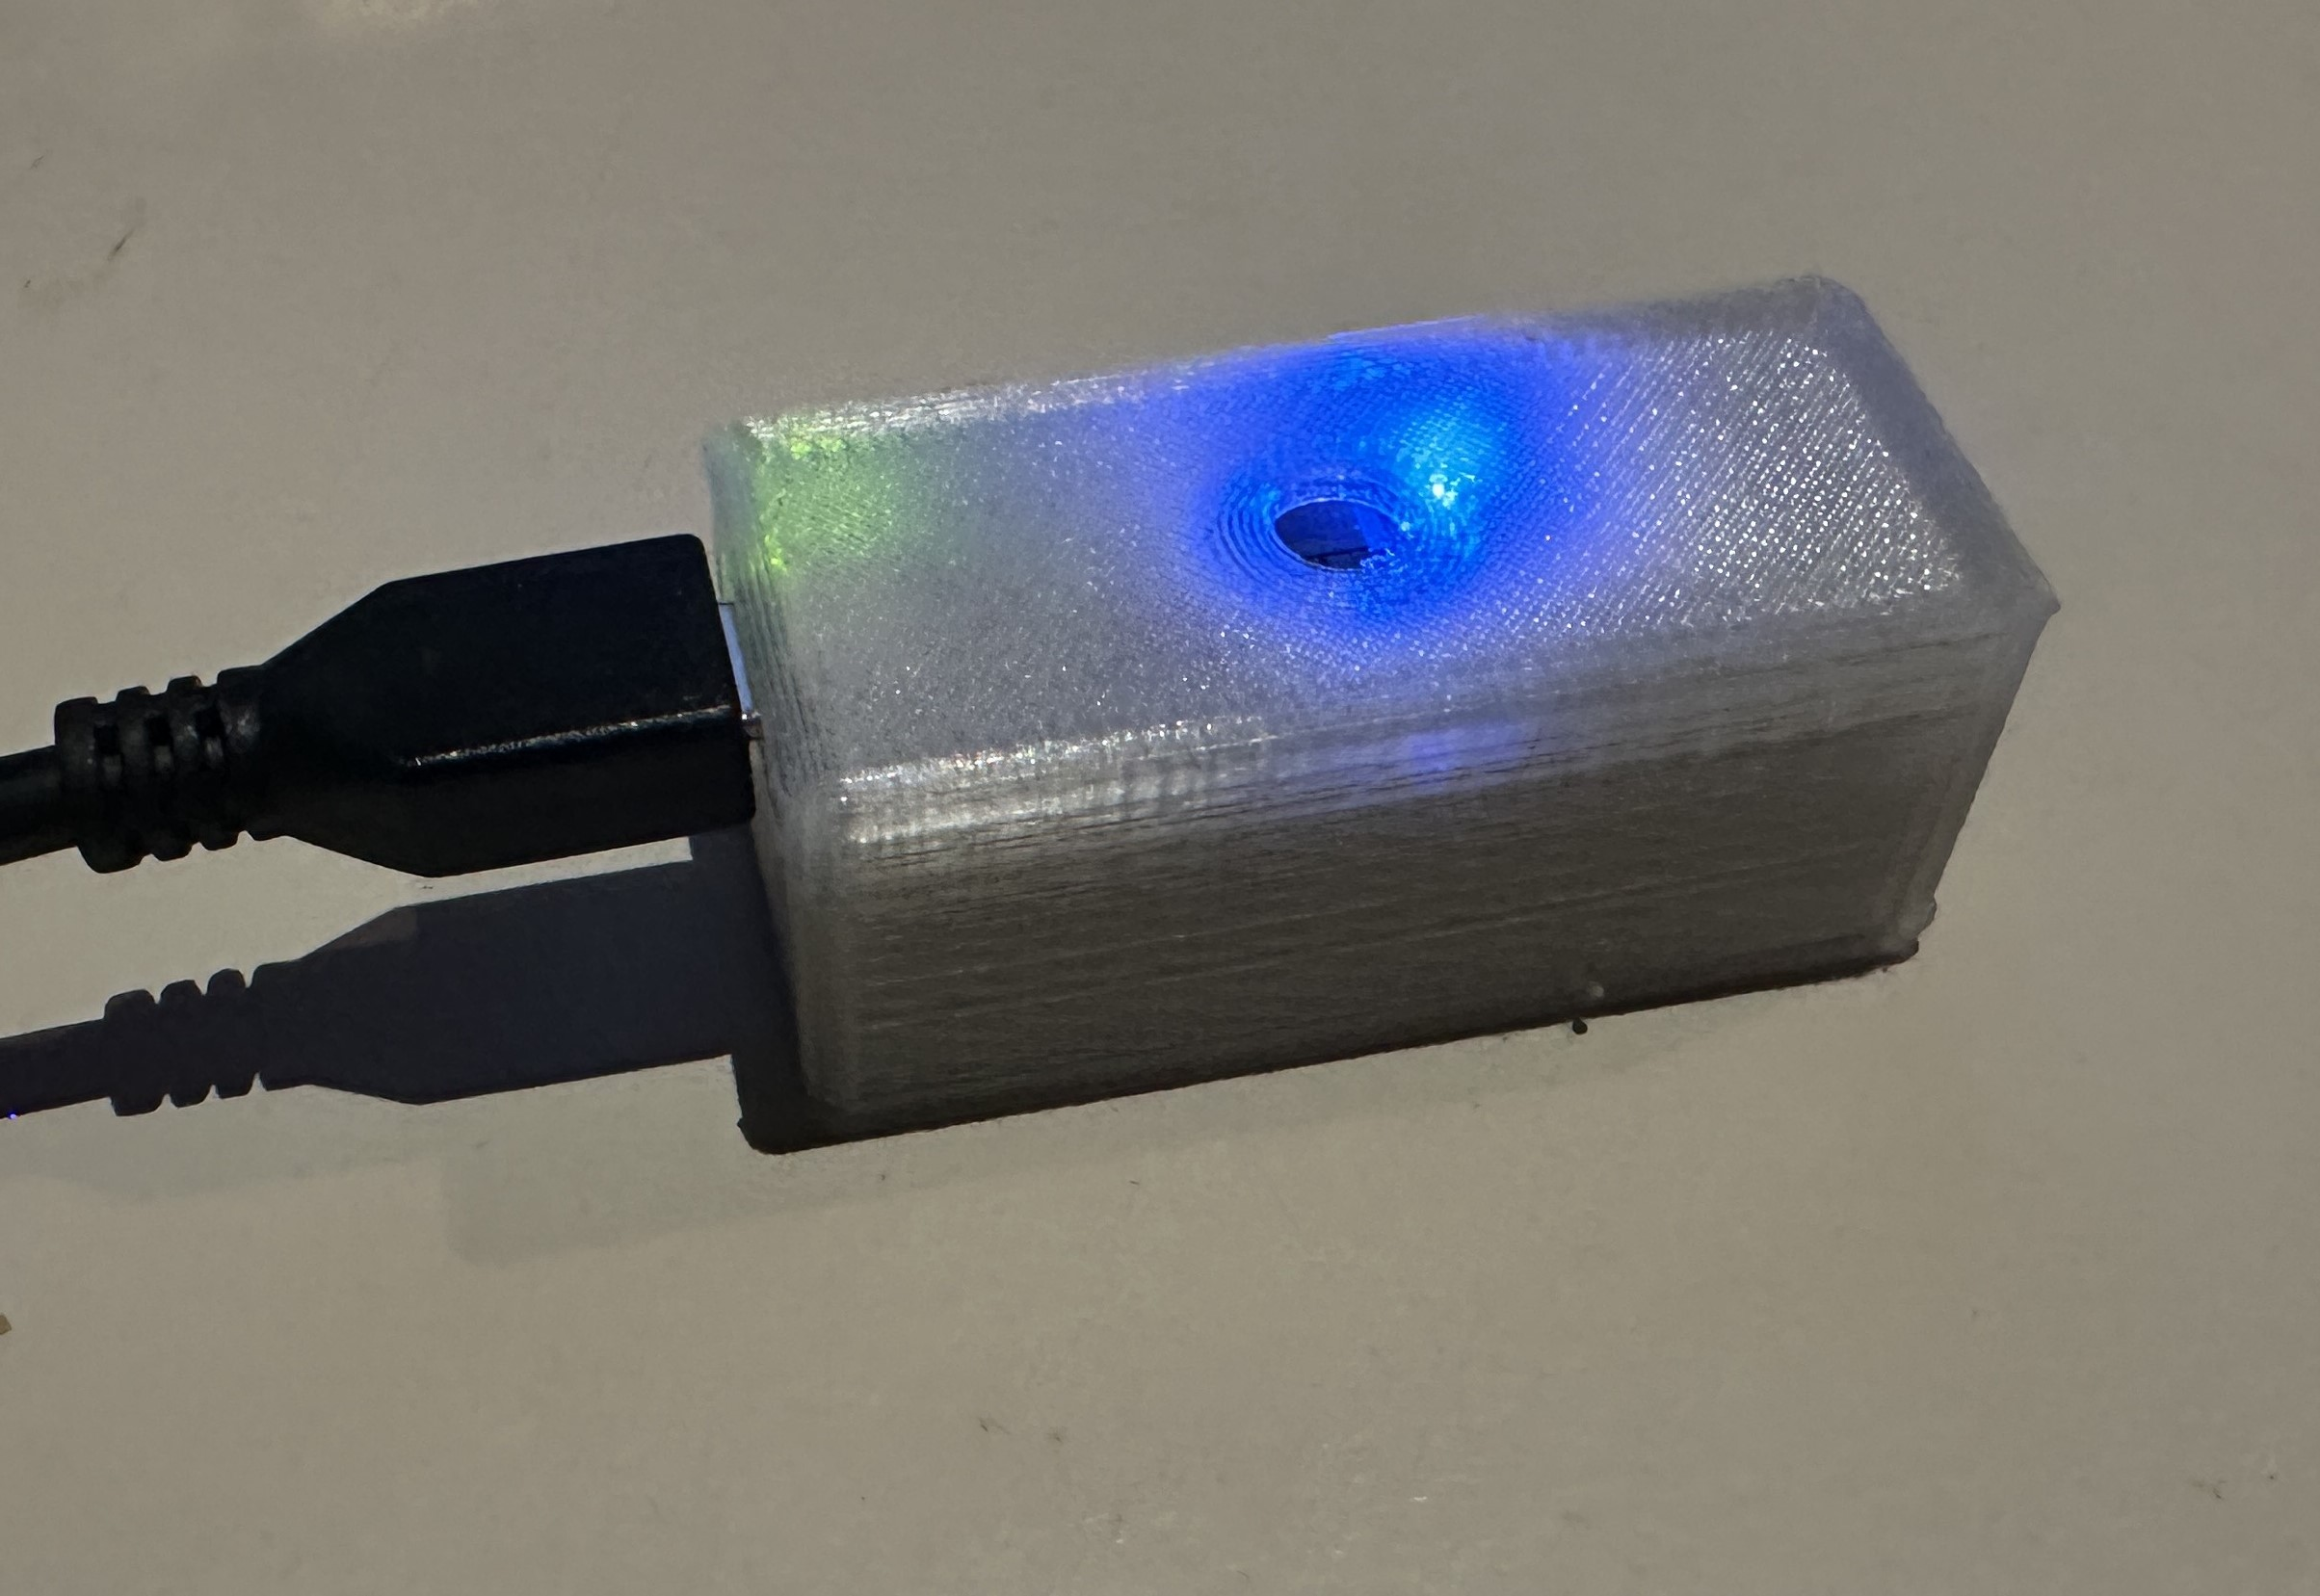
\includegraphics[width=0.6\textwidth]{Images/testhardware/ArduinoBlue}
			\caption{ Response to Unrecognized Keyword} \label{fig:ArduinoBlue}
		\end{figure}
\end{itemize}

\subsection{Reset of Arduino}

When developing and testing your keyword spotting model, we have likely made frequent adjustments to our code. The reset button allows for a quick way to restart the program to test new changes without the need to disconnect and reconnect the board or use the software reset command. This is especially needed for rapid prototyping and debugging.

If our keyword spotting application enters an unexpected state or becomes unresponsive due to a bug or logic error, the reset button can quickly reboot the device, allowing you to resume testing without significant downtime.

Keyword spotting model and the associated signal processing is memory-intensive. If there are any memory leaks or if the program consumes increasing amounts of RAM over time, a reset can clear the memory, helping us to identify and troubleshoot memory-related issues.

	\begin{figure}[h!]
	\centering
	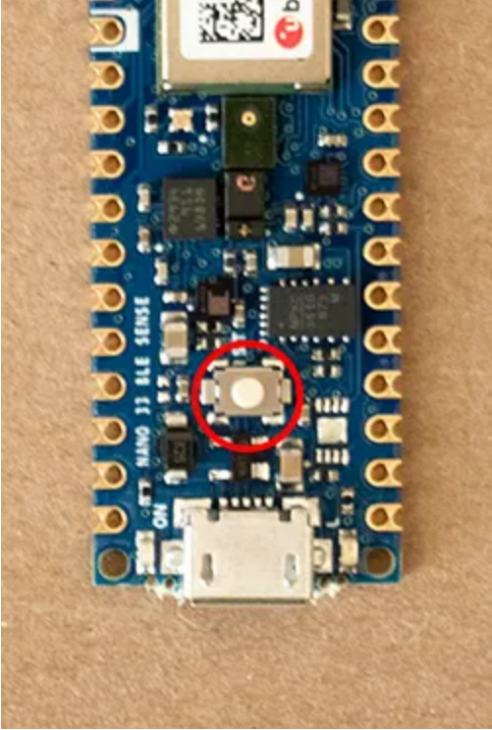
\includegraphics[width=0.5\textwidth]{Images/testhardware/ResetButton}
	\caption{ Reset Button of Arduino} \label{fig:ResetButton}
	\end{figure}
	
\subsection{Hardware Test Documentation}	

\subsubsection{Overview}
This document is designed to guide users through the process of verifying the functionality of the Arduino Nano 33 BLE Sense's digital microphone and built-in LED. These components are essential for developing a keyword spotting system that responds to voice commands with visual feedback.

\subsubsection{Test Environment Setup}

\textbf{Equipment Required}

\begin{itemize}
	\item Arduino Nano 33 BLE Sense board
	\item Computer with Arduino IDE installed
	\item USB cable for connection
	\item Sound source for testing the microphone
	\item A well-lit area to observe LED brightness and color accurately
\end{itemize}

\bigskip

\textbf{Software and Libraries}

\begin{itemize}
	\item Arduino IDE 
	\item PDM library for processing digital microphone input
	\item Basic LED control sketches 
\end{itemize}
	
\textbf{Preparation Steps}

\begin{enumerate}
	\item Arduino IDE Configuration:
	\begin{itemize}
		\item Install the Arduino IDE and open it.
		\item Go to \texttt{Tools > Board} and select "Arduino Nano 33 BLE".
		\item Ensure the correct port is selected under \texttt{Tools > Port.}
	\end{itemize}
	\item Library Installation:
	\begin{itemize}
		\item Go to \texttt{Tools > Manage Libraries…} in the Arduino IDE.
		\item Search for and install the PDM library for microphone input handling.
	\end{itemize}
\end{enumerate}

\subsubsection{Test Procedures}

\begin{enumerate}
	\item \textbf{Digital Microphone Test:}
	The digital microphone on the Arduino Nano 33 BLE Sense is a key component for voice recognition. This test ensures that it can capture sound accurately.

	\textbf{Objective:} To verify the microphone's ability to capture and process audio signals.
	
	\textbf{Procedure:}
	\begin{enumerate}
		\item Load the Test Sketch:
		\begin{itemize}
			\item In the Arduino IDE, open the PDM library's example sketch designed for audio capture.
			\item Review the sketch to understand how audio data is captured and processed.
		\end{itemize}
		\item Upload the Sketch:
		\begin{itemize}
			\item Connect the Arduino Nano 33 BLE Sense to your computer using the USB cable.
			\item Upload the example sketch to the board.
		\end{itemize}
		\item Conduct the Test:
		\begin{itemize}
			\item Open the Serial Monitor in the Arduino IDE to view the output.
			\item Generate a consistent sound toward the microphone (e.g.,YES or NO).
			\item Observe the changes in the Serial Monitor output.
		\end{itemize}	
		
	
\end{enumerate}

\bigskip

\textbf{Expected Outcome:}
\begin{itemize}
	\item The Serial Monitor displays fluctuating numerical values or a waveform pattern that corresponds to the sound input.
	\item Consistent sounds should produce recognizable patterns or consistent data outputs.
\end{itemize}

\item \textbf{Built-in LED Test:}
The built-in LED on the Arduino Nano 33 BLE Sense provides visual feedback, which is crucial for signaling the detection of specific keywords.

\textbf{Objective:} To confirm that the built-in LED can display various colors and respond to voice commands.

\textbf{Procedure:}
\begin{enumerate}
	\item Prepare the LED Test Sketch:
	\begin{itemize}
		\item Write or modify a simple sketch that sequentially lights up the LED in different colors (red, green, blue) with a pause between each color.
		\item Include commands to control the LED's brightness if necessary.
	\end{itemize}
	\item Upload the Sketch:
	\begin{itemize}
		\item With the Arduino connected, upload your LED test sketch to the Nano 33 BLE Sense.
	\end{itemize}
	\item Observe the LED Behavior:
	\begin{itemize}
		\item Watch the LED as the sketch runs. Note the color changes and any variations in brightness.
	\end{itemize}
\end{enumerate}

\bigskip

\textbf{Expected Outcome:}
\begin{itemize}
	\item The LED cycles through the specified colors clearly and smoothly.
	\item Adjustments in brightness are noticeable if included in the test sketch.
\end{itemize}

\item \textbf{Reset Functionality Test:}

\textbf{Objective:} Ensure the reset button correctly reboots the board without issues.

\textbf{Procedure:}
\begin{itemize}
	\item While the Arduino Nano 33 BLE Sense is connected and running any sketch, press the reset button on the board.
	\item Observe the behavior of the board and any connected peripherals or indicators (e.g., LEDs).
\end{itemize}

\bigskip

\textbf{Expected Outcome:} The board resets and restarts the sketch from the beginning, as indicated by the operational sequence of LEDs or serial output, confirming the reset functionality. 
\end{enumerate}

\subsubsection{Troubleshooting}

\begin{itemize}
	\item If any component does not perform as expected, check connections, ensure correct board selection in the Arduino IDE, and verify that all necessary libraries are installed and up to date.
	\item For the digital microphone test, ensure no other program is using the Serial Monitor and adjust the volume of the sound source if necessary.
\end{itemize}

\subsubsection{Conclusion}

This document provides a structured approach to testing the critical hardware components of the Arduino Nano 33 BLE Sense in the context of a keyword spotting project. Successful completion of these tests confirms the hardware's readiness for development and deployment of the application.

\section{Data Quality in Hardware Description}

Within the hardware description of our project utilizing the Arduino Nano 33 BLE Sense, we delve into several facets related to data quality:

\begin{enumerate}
	\item \textbf{Precision of Sensors:}
	
	The integrated sensors on the Arduino Nano 33 BLE Sense board deliver precise measurements of environmental parameters, encompassing motion, orientation, temperature, humidity, and pressure.
	
	\item \textbf{Sampling Rate:}
	
	The sensors' sampling rate determines the frequency of data collection. The Arduino Nano 33 BLE Sense board supports high sampling rates, facilitating real-time data acquisition at \textless{}some frequency\textgreater{} Hz.
	
	\item \textbf{ Noise Mitigation:}
	
	Despite potential noise sources like sensor imperfections and external interference, the data's noise level is minimized through adept calibration and filtering techniques.
	
	\item \textbf{Efficient Data Transmission:}
	
	Sensor data is efficiently transmitted from the Arduino Nano 33 BLE Sense board to other devices through wireless communication protocols like Bluetooth Low Energy (BLE), ensuring minimal latency and reliable delivery.
	
	\item \textbf{Data Integrity Assurance:}
	
	Measures are taken to guarantee the integrity of sensor data during transmission and processing. Employing error detection and correction mechanisms helps identify and rectify instances of data loss or corruption.\cite{TensorFlow:2023}
	
	\item \textbf{Optimized Power Consumption:}
	
	The Arduino Nano 33 BLE Sense board exhibits low power consumption, rendering it suitable for battery-powered applications. Power requirements are meticulously managed to extend battery life while sustaining continuous data acquisition.
\end{enumerate}

\subsection{Specifications of Arduino Nano 33 BLE Sense}



\subsubsection*{NINA B306 Module}
\begin{enumerate}[label=\arabic*.]
	\item Processor:
	\begin{itemize}[label=-]
		\item 64 MHz Arm® Cortex-M4F (with FPU)
		\item 1 MB Flash + 256 KB RAM
	\end{itemize}
	\item Bluetooth® 5 multiprotocol radio:
	\begin{itemize}[label=-]
		\item 2 Mbps
		\item +8 dBm TX power
		\item -95 dBm sensitivity
		\item 4.8 mA in TX (0 dBm)
		\item 4.6 mA in RX (1 Mbps)
		\item Integrated balun with 50 Ohm single-ended output
		\item IEEE 802.15.4 radio support
	\end{itemize}
	\item Peripherals:
	\begin{itemize}[label=-]
		\item 12 Mbps USB
		\item NFC-A tag
		\item Arm CryptoCell CC310 security subsystem
		\item QSPI/SPI/TWI/I2S/PDM/QDEC
		\item 32 MHz SPI
		\item Quad SPI interface 32 MHz
		\item 12-bit 200 ksps ADC
		\item 128 bit AES/ECB/CCM/AAR co-processor
	\end{itemize}
\end{enumerate}

\section{Constraints}
\subsubsection{Arduino Nano 33 BLE Sense}
\begin{itemize}[label=--]
	\item Operating Voltage: 3.3V
	\item Power Consumption:
	\begin{itemize}[label=--,leftmargin=*]
		\item Maximum 15mA in low power mode
		\item Maximum 60mA in active mode
	\end{itemize}
	\item Operating Temperature Range: -40°C to 85°C
	\item Memory Constraints: 1 MB Flash + 256 KB RAM
	\item Communication Interfaces: USB, Bluetooth 5, NFC-A, SPI, I2C, QSPI, etc.
\end{itemize}


\subsubsection*{Actuators}
\begin{itemize}[label=--]
	\item RGB LEDs:
	\begin{itemize}[label=--,leftmargin=*]
		\item Power Requirements: Voltage, Current
		\item Operating Temperature Range
	\end{itemize}
	\item Buzzer/Speaker:
	\begin{itemize}[label=--,leftmargin=*]
		\item  Voltage, Current, Sound Output Levels
	\end{itemize}
	
\end{itemize}

\subsubsection*{Power Supply}
\begin{itemize}[label=--]
	\item Input Voltage Range: Specify the acceptable input voltage range.
	\item Power Consumption: Estimate the overall power consumption of the system.
\end{itemize}

\subsubsection*{Physical Constraints}
\begin{itemize}[label=--]
	\item Size and Dimensions: Ensure compatibility with the project enclosure or housing.
	\item Mounting Requirements: Specify any specific mounting requirements for the components.
\end{itemize}

\subsubsection*{Environmental Constraints}
\begin{itemize}[label=--]
	\item Environmental Protection: Ensure components are suitable for the intended environmental conditions (e.g., moisture resistance, dust resistance).
	\item Operating Conditions: Specify any limitations or special considerations for operating in certain environments.
\end{itemize}

\section{Dimensions of the Arduino Nano 33 BLE Sense}


The Arduino Nano 33 BLE Sense is a compact board with dimensions of 45mm x 18mm. This small form factor makes it ideal for wearable devices and compact projects. However, despite its small size, it comes packed with a variety of sensors and features, making it a versatile choice for many projects.
Please note that these dimensions are for the board without headers. If you're using a version with headers or if you're adding additional components to the board, this could affect the overall dimensions of your hardware setup. Always refer to your specific board and components for the most accurate dimensions. \cite{Arduino:2023}


  
